\documentclass[twocolumn, longbibliography]{revtex4-2}

\usepackage{amsmath}
\usepackage[dvipsnames]{xcolor}
\usepackage{hyperref}
\hypersetup{
	colorlinks=true,
	linkcolor=blue,   
	urlcolor=blue,
}
\usepackage{graphicx}

\newcommand{\note}[1]{\textcolor{red}{#1}}
\newcommand{\outline}[1]{\textcolor{Plum}{#1}}
\newcommand{\TC}{\text{TC}}
\newcommand{\nn}{\nonumber\\}
\newcommand{\cond}{\text{cond}}
\newcommand{\RBH}{\text{RBH}}
\newcommand{\tdtf}{\text{3d3f}}
\renewcommand{\l}{\ell}
\newcommand{\ket}[1]{\left|#1\right\rangle}

\begin{document}
	
\title{Symmetry-protected self-correction in Walker-Wang models}
\author{charlie}
	
\begin{abstract}
The discovery that quantum error correcting codes can be self-correcting in four spacial dimensions has led to much interest in recent years into whether the same is possible in three spacial dimensions. There are restrictions under which a $d\leq 3$ model can be self-correcting, but these restrictions are all non-physical in some sense. Recently an additional such restriction has been identified, that of imposing a higher-form symmetry. Higher-form symmetries are local rather than global, so this is a very strong constraint. 
We also show that this property extends to a class of 3d topological models. In particular, any confined Walker-Wang model can be made self-correcting by imposing a one-form symmetry. 
\end{abstract}
	
\date{\today}
	
\maketitle
	
\section{Introduction}
	
\outline{Error correction using topological phases}
	
The introduction of the toric code showed that topological phases could be used to store quantum information even when using noisy physical qubits. 
	
\outline{2d toric $\longrightarrow$ active correction, T=0. 4d toric $\longrightarrow$ passive correction, T>0.}
	
In the 2d toric code, errors must actively be corrected, while it was later shown that the 4d toric code can store quantum information under passive correction.
	
\outline{Switch to condensed matter perspective.}
	
Error-correcting stabilizer codes can be studied from the condensed matter perspective by defining a Hamiltonian that is the sum of all the stabilizers. In this language, the difference between the 2d and the 4d toric codes is that the 4d toric code has topological order at nonzero temperatures, while the 2d toric code only has topological order at $T=0$.
	
The ground states of the 2d toric code are loop gasses, in that they can be written as a product of closed loop operators acting on a reference state. The ground states of the 4d toric code are membrane condensates in the same sense. We will refer to these loops and membranes as gauge structures, because they are gauge-equivalent on the ground-space manifold. Gauge structures are always closed.
	
Once characteristic of topological order is a topology-dependent ground-state degeneracy. Nontrivial operators on the ground-space manifold are non-contractible gauge structures. For example in the 2d toric code they are non-contractible loops. 
	
Unhappy stabilizers appear as excitations above the ground state, appearing at the boundaries of open versions of gauge structures. For the 2d toric code these are point-like excitations on the ends of strings, while in the 4d toric code they are line-like excitations on the boundary of open membranes. \note{Fix this terminology.}
	
Since we live in three spacial dimensions, it is natural to study the 3d toric code. Unlike the 2d and 3d versions which are self-dual, this model has one sector with stabilizers that look like those of the 2d toric code and one with stabilizers that look like those of the 4d toric code. As such, its ground states can be written as loop gasses or membrane gasses.
	
All three toric codes have topological order at zero temperature, but have different nonzero temperature behavior. The 3d toric code remains topologically ordered for small nonzero temperatures, but the order is classical. From the information theory perspective this means the code can protect a classical probabilistic bit (a pbit) but not a qubit. 
	
In both the 2d and 3d toric codes the nonzero temperature behavior can be traced to the finite energy barrier. The bath can lend a constant amount of energy to create two point defects and then transport them at no energy cost across the system. When they annihilate they leave behind a non-contractible gauge structure, which we said acted nontrivially on the ground space. For the 4d toric code, the bath must create a membrane that stretches across the system. Since energy cost of open membranes is linear in perimeter, the energy barrier to membrane operators is linear in system size.
	
With this motivation, considerable work has been done to try to find systems with unbounded energy barriers, and a number have been found, such as the X-cube model, Haah's cubic code, and Michnicki's welded code. They are collectively referred to as marginally self-correcting. It is worth noting that all of these codes have an energy barrier that grows less than linearly, either logarithmically (X-cube and Haah's) or polynomially (Michnicki's).
	
However, it has been shown that the bath still disorders these models at any $T>0$. As in the 2d and 3d toric codes, the marginally self-correcting models have point-like excitations. At nonzero temperature these excitations exist at some finite density, leading to an energy barrier that is bounded by a function of the temperature.
	
Accordingly, a new goal is to find a system whose energy barrier $\Delta$ grows without bound, even for some $T>0$. Note that this is still not directly probing the memory time $\tau$, but that the community has found no systems with unbounded $\Delta$ and bounded $\tau$. In all known models the bound on energy barrier comes from the finite density of point excitations.
	
\note{Does the 4d toric code have an unbounded energy barrier at nonzero temperature?} 
	
A recent proposal directly removes the point excitations from the picture. The authors enforce that the stabilizers whose excitations are point-like are satisfied, so that there can be no point excitations at all. This is achieved by enforcing what is called a 1-form symmetry.
	
Consider the 2d toric code. If no point excitations are allowed, then the bath cannot apply the string operators through a series of local operations. Of course, then no logical operations can be performed \note{transversally}. Ref.~\cite{RobertsBartlett} instead creates a code that, when the symmetry is enforced, behaves like the 4d toric code in that logical operators can be applied transversally but with a large enough energy barrier that the bath applies them with probability 0 in the thermodynamic limit.
	
In this \note{paper} we show how to achieve the same results using the 3d 3-fermion model, a specific example of a confined Walker-Wang model. This prescription should work for any confined Walker-Wang model. We will then compare our result to one of the realizations in Ref.~\cite{RobertsBartlett}, ending with some discussion of future work.
	
\note{Terminology: points, lines, loops, strings, membranes...}
	
\section{Self-correction in the three-fermion model}
	
In this section we will first define the 3d 3-fermion model in the absence of the protecting symmetry and show it is not self-correcting. We then define the 1-form symmetry and show what gauge structures and excitations can exist in its presence. Finally, we show the 3d 3-fermion model is self-correcting in the presence of the 1-form symmetry.
	
\subsection{The model}
	
\outline{Two copies of 3d toric}
	
The three-fermion model can be thought of as two copies of the 3d toric code, ``twisted" together so that flux from one code confines the point-like excitations of the other. To be concrete, consider a cubic lattice with two qubits on each edge. We will refer to them as $\sigma$ and $\tau$ qubits, and they will be acted on by Pauli matrices written as $\sigma^\alpha$ and $\tau^\alpha$ respectively, $\alpha = x,z$. Two independent toric codes would have the Hamiltonian 
\begin{align}
H_{\TC} &= -\sum_vA_v^{\sigma}-\sum_vA_v^{\tau}-\sum_fB_f^{\sigma}-\sum_fB_f^{\tau},\nn
A_v^{\sigma} &= \prod_{e\in \partial^*v}\sigma_e^x, \qquad B_f^{\sigma} = \prod_{e\in\partial p}\sigma_e^z,\nn
A_v^{\tau} &= \prod_{e\in \partial^*v}\tau_e^x, \qquad B_f^{\tau} = \prod_{e\in\partial p}\tau_e^z, 
\label{eqn:toric}
\end{align}
so that the two codes do not talk to each other at all. We will refer to the two types of terms as vertex terms and face terms. 
	
In each code there are line-like operators with point-like excitations and membrane operators with loop-like excitations. We will call flipped $A_v^\sigma$ terms $e$-particles and flipped $A_v^\tau$ terms $m$-particles. Since flipped $B_f^\sigma$ and $B_f^\tau$ terms naturally come in dual strings, we will refer to them as $\sigma$-flux and $\tau$-flux, respectively. $e$-particles see $\sigma$-flux and $m$-particles see $\tau$-flux. Finally, $e$-particles exist on the ends of $e$-lines, $\sigma$-flux lives on the end of $\sigma$-membranes, etc.
	
\outline{Twist them together}
	
We can twist the codes together by dressing the face operators to create the 3d 3-fermion Hamiltonian,
\begin{align}
H_{\tdtf} &= -\sum_vA_v^{\sigma}-\sum_vA_v^{\tau}-\sum_fB_f^{\sigma}-\sum_fB_f^{\tau},\nn
A_v^{\sigma} &= \prod_{e\in \partial^*v}\sigma_e^x, \qquad B_f^{\sigma} = \tau_O^x\prod_{e\in\partial p}\sigma_e^z,\nn
A_v^{\tau} &= \prod_{e\in \partial^*v}\tau_e^x, \qquad B_f^{\tau} = \sigma^x_U\prod_{e\in\partial p}\tau_e^z, 
\label{eqn:3d3f}
\end{align}
where the edges O and U lie ``over" and ``under" the given face. Labeling these edges requires a choice of 2d projection. This is shown in Fig.~\ref{fig:legs}, where the $O$ edges are red and the $U$ edges are blue. \note{These decorations are different than in Burnell et al. I think they result in the same physics, but should check. Use App. B of Burnell.} The result of this decoration is that, for example, a string of $\sigma^z$ operators that would usually create two deconfined $e$ particles now also creates a string of $\tau$-flux. We will see this means point excitations are confined in the bulk.
	
\begin{figure}
\centering
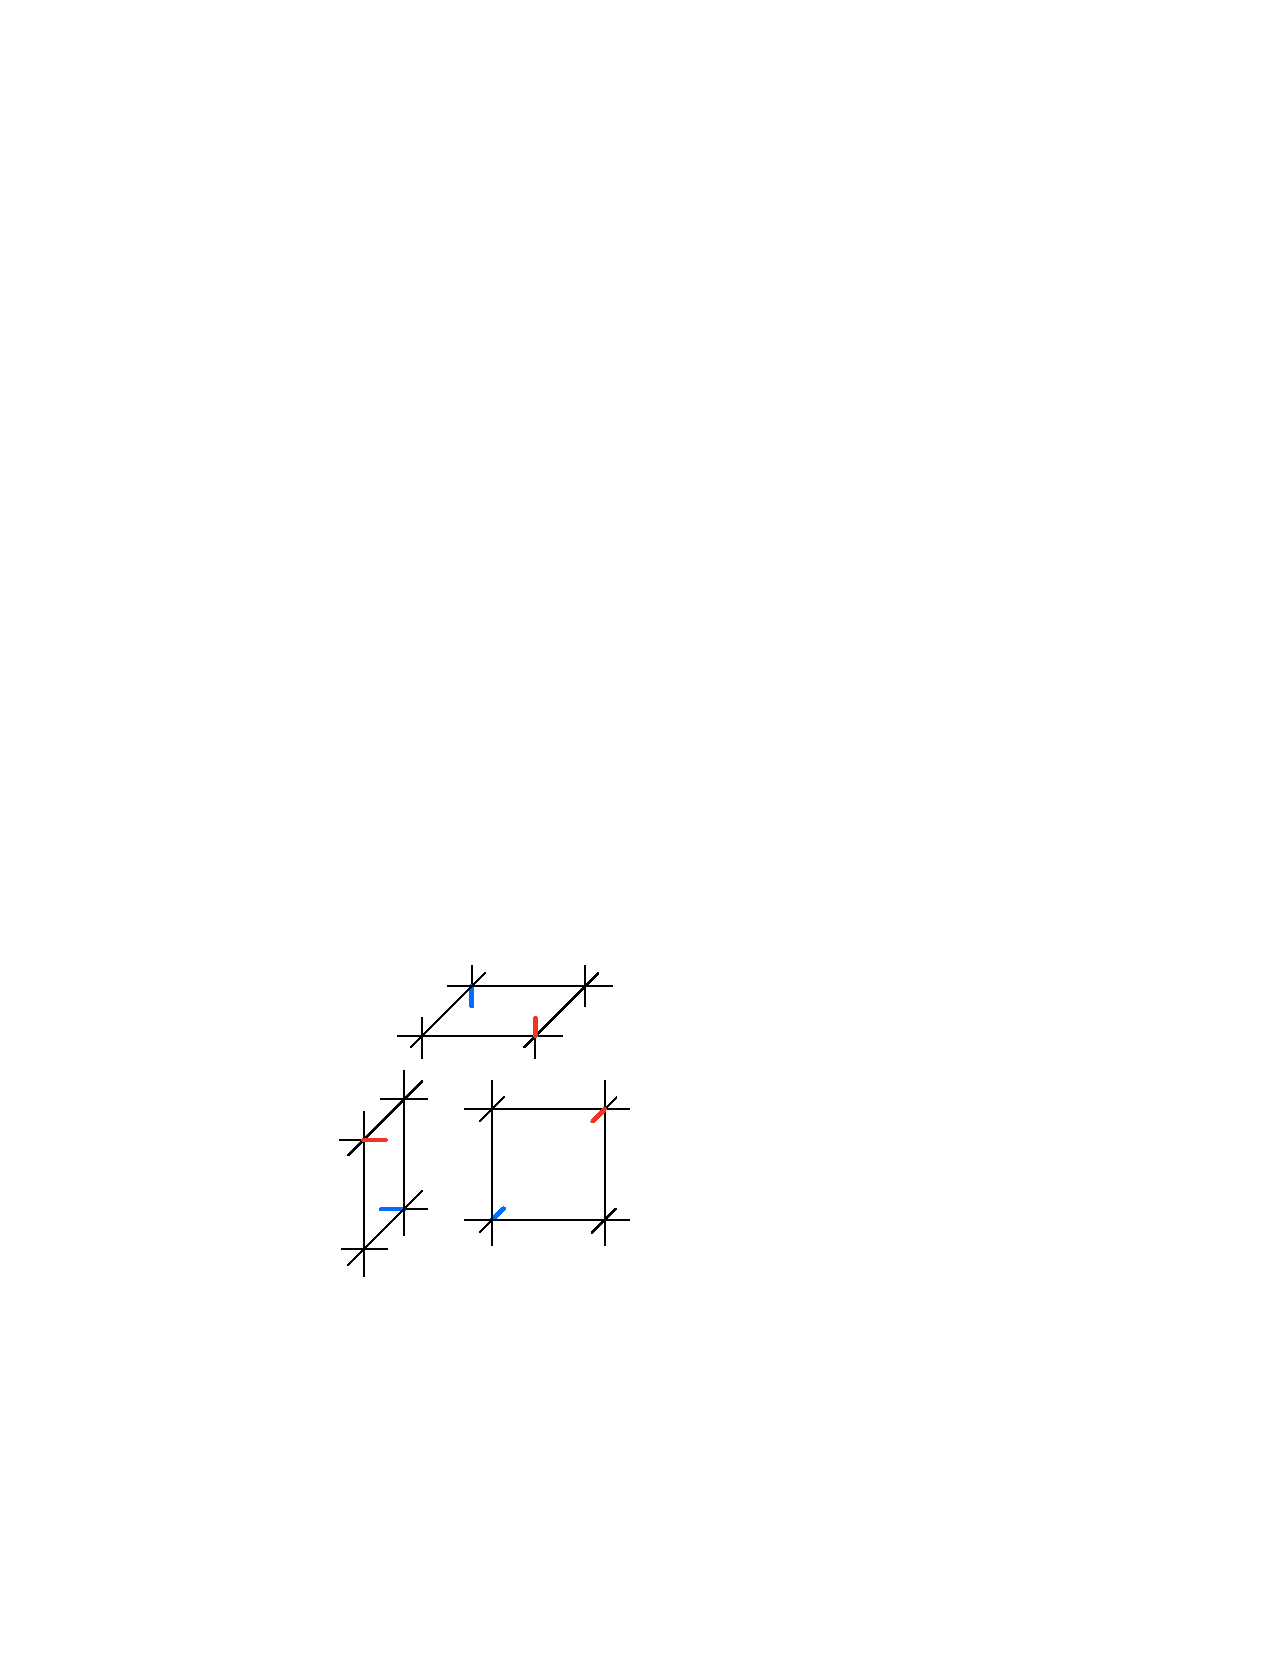
\includegraphics[width=\linewidth]{legs}
\caption{Once we have fixed a projection, we can choose the $O$ and $U$ legs to be the ones the lie over and under the plaquette. }
\label{fig:legs}
\end{figure}
	
\outline{Bulk properties}
	
Membrane operators are the same as they were in the toric code, being dual membranes of $\sigma^x$ or $\tau^x$ operators. However, a line operator consisting of $\sigma^z$ or $\tau^z$ now creates flux excitations along its entire length in addition to creating point excitations on its ends. Thus point excitations in the bulk are always linearly confined by flux.
	
The flux that confines the point particles is the same as the flux on the boundary of membranes, in that both are dual lines of flipped face operators. Once a line operator separates two point excitations, a membrane operator can transport the flux elsewhere, with the constraint that the flux terminates on the points. The resulting composite operator can alternatively be seen as a membrane operator where some of the flux has been removed by a line operator. This composite membrane-line operator will be important in Sec.~\ref{sub:ener}.
	
The 3d 3-fermion model contains no topological order in the bulk. One explanation for this is that point particles are confined. Thus there is no way to transport point particles across the system and return to the ground space. The result is that the 3d 3-fermion model is trivial when defined on manifolds without boundary.
	
On a manifold with a boundary, it is easy to terminate the code in a way that creates topological order. To do this, truncate the lattice using ``smooth" boundary conditions, so that no legs are sticking out. Then truncate any stabilizers to include all their operators that act on qubits that haven't been removed. Such stabilizers are shown in Fig.~\ref{fig:bdyops} The result is a 2d $\mathbf{Z}_2$ topological order where all anyons are fermions~\cite{BurnellSoluble}.
	
\begin{figure}
\centering
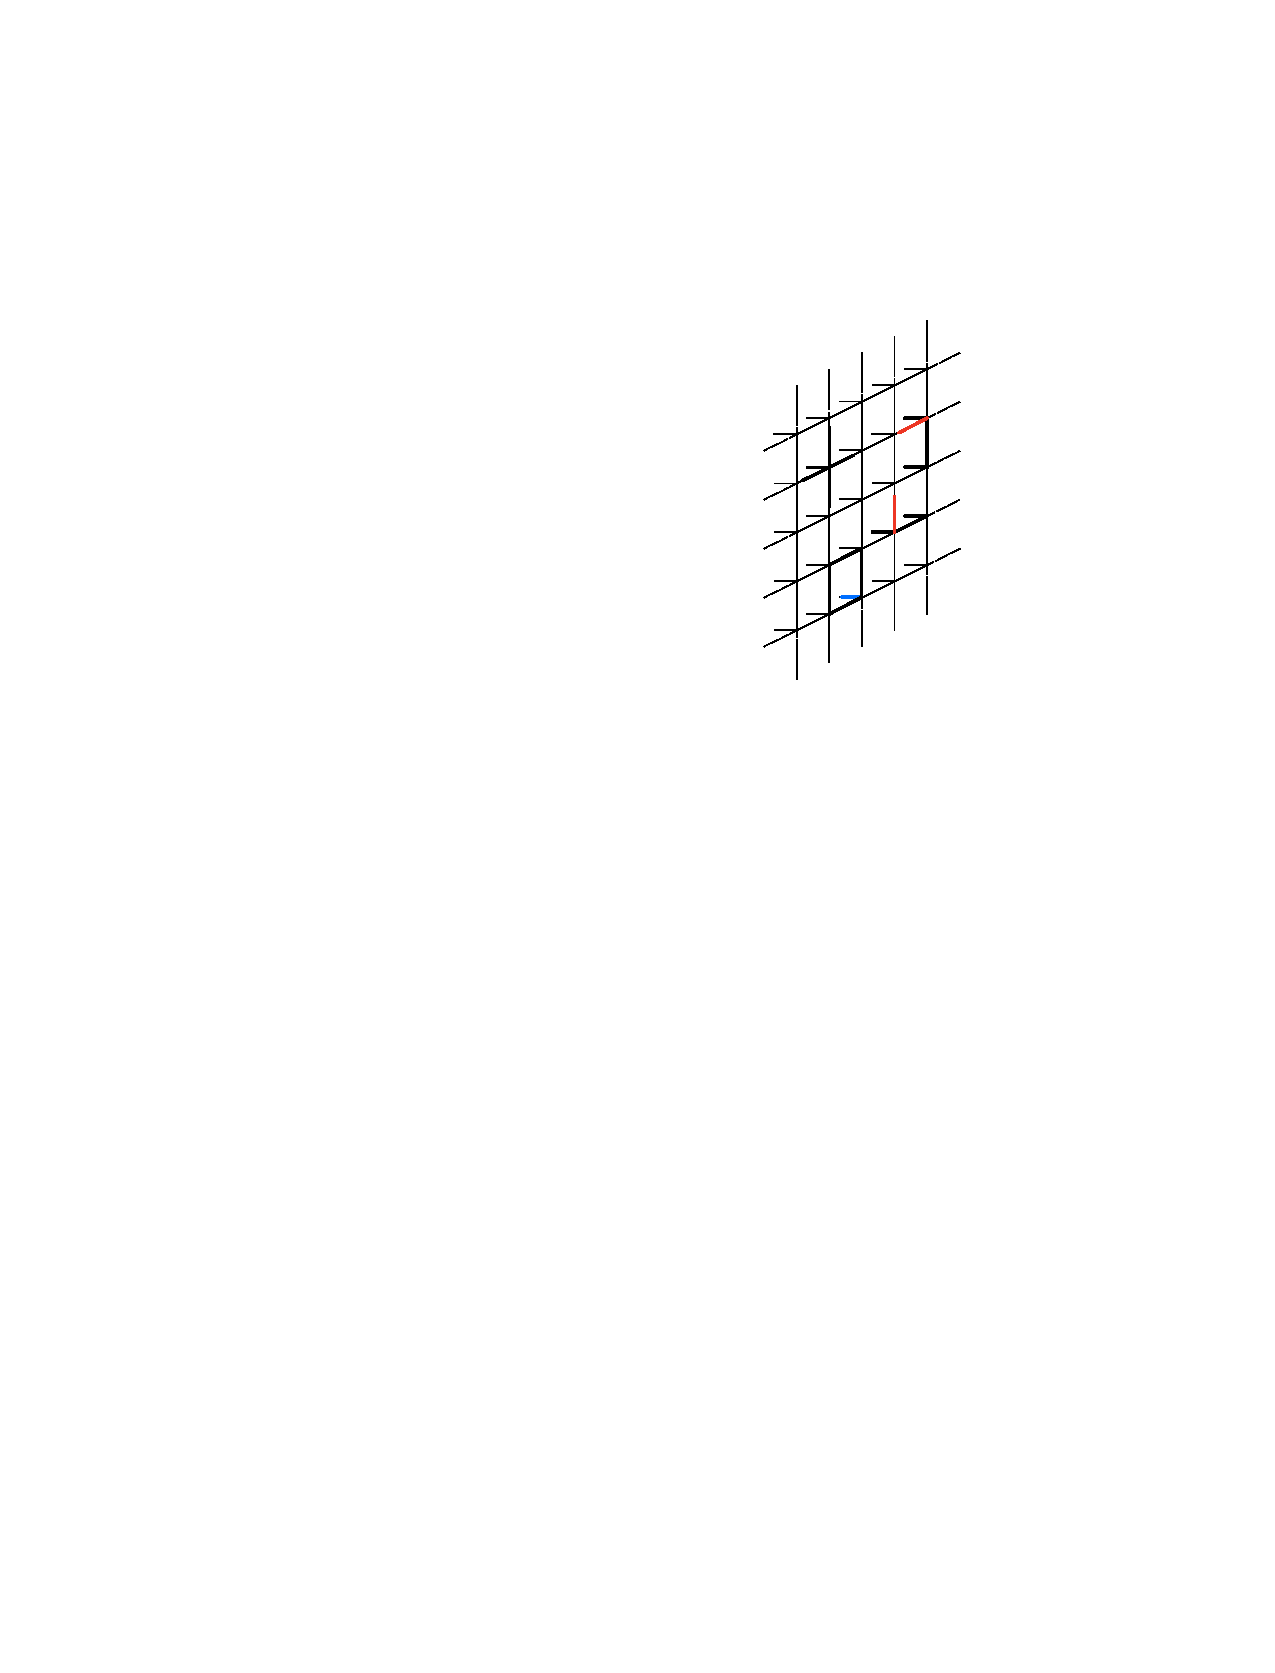
\includegraphics[width=.6\linewidth]{bdyops}
\caption{The stabilizers on the boundary are truncated versions of the ones in the bulk. Red represents $O$ edges and blue represents $U$ edges. The two face operators that reach into the bulk each have a $U$ edge that is not shown, while the boundary face operator does not have any $O$ edge.}
\label{fig:bdyops}
\end{figure}
	
Since the bulk is trivial, we should think of this phase as being equivalent to any trivial bulk with a 2d $\mathbf{Z}_2$ topological order attached to the boundary. We will later show how to use the 1-form symmetry to couple the bulk and the boundary.
	
We will consider the 3d 3-fermion model defined on a lattice with topology $T^2\times I$, where $T^2$ is the torus and $I$ is the unit interval $[0,1]$. This can be constructed from a cubic lattice by identifying the boundaries in the $x$- and $z$-directions, so that the only true boundaries are at $y=0,1$. We will refer to these as the the right and left boundaries, respectively. Each boundary supports two qubits. \note{FIGURE.}
	
Since the topological order exists on the boundary, there must be logical operators supported only on boundary qubits. These are the deconfined line operators
\begin{align}
S\dots
\end{align}
which do not create flux along their length. We can think of the flux as having been fused into the boundary.

\begin{figure}
\centering
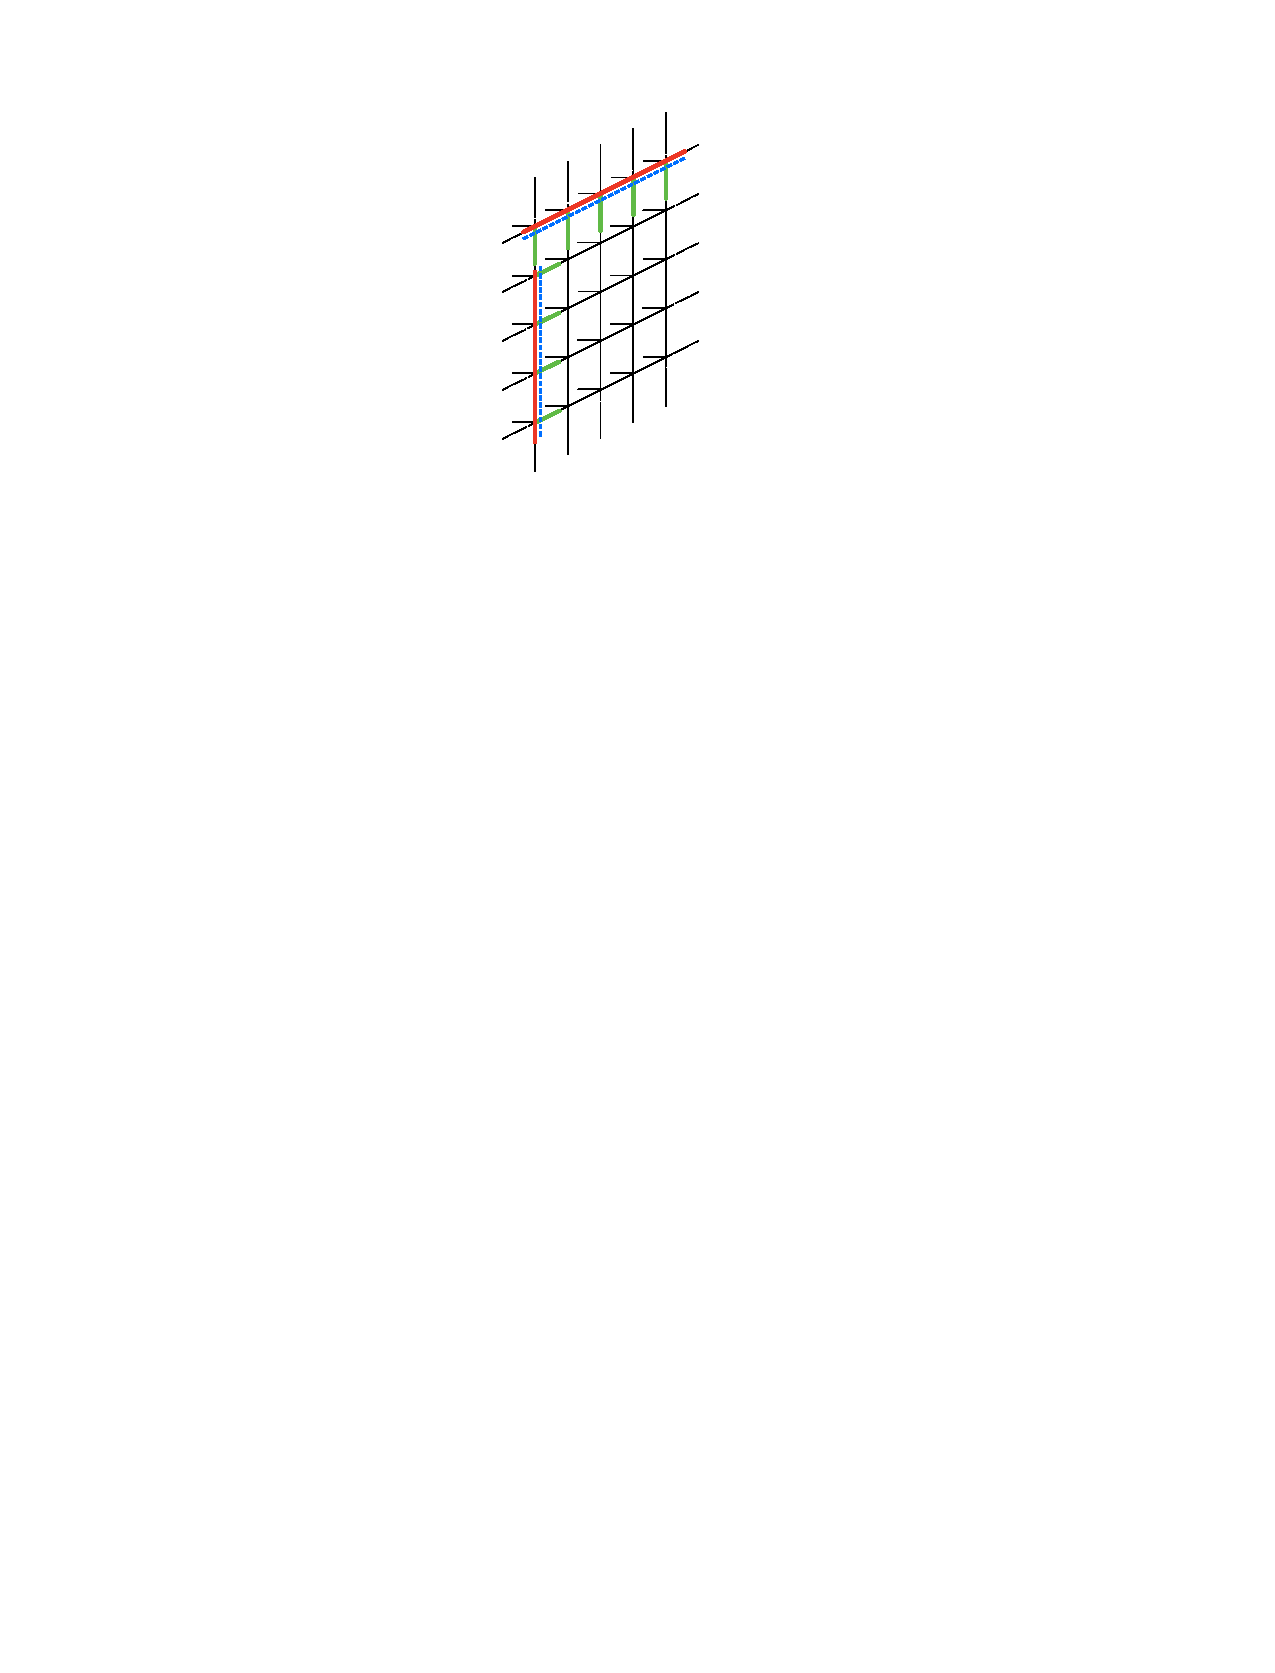
\includegraphics[width=.5\linewidth]{deconf}
\caption{It is possible to create deconfined line operators on the boundary. For $S\dots$ the green edges are \dots}
\label{fig:deconf}
\end{figure}
	
\outline{Structure of topological order/ which types of operators are logical}
	
The bath is able to transport deconfined point particles across the system at any temperature above zero. This is the case in both the 2d and 3d toric code. In our case, all logical operators can be applied by transporting a deconfined point excitation. 3D3F cannot store any information, even classical, at nonzero temperature. The same is true of confined Walker-Wang models in general. 
	
\subsection{Enforcing a 1-form symmetry}
	
\outline{Definition of higher-form symmetry}
	
Here we define $p$-form symmetries, which for $p>0$ are called higher-form symmetries. A $p$-form symmetry consists of symmetry operators each associated with a closed $(d-p)$-dimensional submanifold of our space. The simplest examples, 0-form symmetries, are just ordinary global symmetries. They act on closed $d$-dimensional submanifolds, so they have to act on the whole space.
	
It may be unintuitive to think about symmetry operators that act on lower dimensional submanifolds. But toric codes actually provide convenient settings to think about them. In the 3d toric code, arbitrary products of vertex operators form (dual) membrane operators. These operators commute with the Hamiltonian, so they form a symmetry. The are defined on $(2=d-1)$-dimensional submanifolds, so they form a 1-form symmetry. The face terms form a 2-form symmetry, but we are not concerned with that here.
	
\outline{$\langle A_v\rangle$ is a 1-form symmetry}
	
Since the vertex terms were not affected when we twisted our toric codes together, the 3d 3-fermion model inherits the same 1-form symmetry. In particular, the symmetry group is 
\begin{align}
G = \langle A_v^\sigma |v\in \Delta_0 \rangle\times
\langle A_v^\tau |v\in \Delta_0\rangle,
\end{align}
the group generated by all the vertex terms.
	
\outline{Enforcing prevents points, and therefore open strings}
	
\outline{Allows closed strings, open membranes, closed membranes. Recall local decomposition and informal energy barrier}
	
We enforce the 1-form symmetry by requiring that all $A^\sigma_v$ and all $A^\tau_v$ operators be satisfied at all times. This removes point-like excitations and open strings from the lattice, so line-like operators cannot be symmetrically locally decomposed.
	
\outline{Partial enforcement: membrane-strings if endpoints are outside protected area}
	
Since the deconfined strings only exist on the boundary, it is tempting to only enforce the symmetry on the boundary. However we can then apply a dual string of, say, $\sigma^x$ operators on the boundary. This creates $\sigma$ flux that can be terminated in the bulk by a $\tau^z$ string. This type of operator is an example of the composite membrane-string operators introduced earlier. In more generality, if the 1-form symmetry is enforced to a distance $d_1$ from the boundary, a composite membrane-string nontrivial logical operator can be symmetrically decomposed with energy barrier $\Delta=\mathcal{O}(d_1)$.
	
\subsection{Diverging symmetric energy barrier} \label{sub:ener}
	
Since we assume the bath couples to the system locally, it can only apply a logical operator by decomposing it into a series of local operations. These local operations generically create excitations in the system. Informally, the energy barrier is the energy of these excitations. We define the energy barrier more formally following Ref.~\cite{RobertsBartlett}.
	
First assume the bath couples to the system through local Pauli operators. Let $\bar{\l}$ be a (nontrivial) logical operator. Define the local decomposition of $\bar{\l}$ as a series of operators $\mathcal{D}(\bar{\l}) = \{\l^{(k)}| k = 1,\dots,N\}$, where $\l^{(1)}=I$ and $\l^{(N)}=\bar{\l}$. Furthermore, $\l^{(k)}$ and $\l^{(k+1)}$ differ only by a local Pauli operator. Since every Pauli operator either commutes or anti-commutes with each stabilizer, each of the $\l^{(k)}$ anticommutes with a finite number of stabilizers.
	
If $\ket{\psi_0}$ is a ground state of the Hamiltonian, then $\l^{(k)}\ket{\psi_0}$ is an eigenstate with energy $E^{(k)}$. Define the energy barrier for this particular local decomposition as
\begin{align}
\Delta_{\mathcal{D}(\bar{\l})}=\max_k(E^{(k)}-E_0),
\end{align}
where $E_0$ is the ground state energy. Then the energy barrier for the system is
\begin{align}
\Delta = \min_{\bar{\l},\mathcal{D}(\bar{\l})}\Delta_{\mathcal{D}(\bar{\l})},
\end{align}
where the minimization is taken over all local decompositions of all logical operators. Thus the system energy barrier $\Delta$ can be thought of as the minimum amount of energy that the bath must supply to perform a nontrivial logical operation.
	
\outline{Calculation of energy barrier}
	
We now turn our focus to the $L\times L\times L$ 3d 3-fermion model, with the 1-form symmetry enforced within distance $W$ of the boundary. In this case the minimum energy barrier comes from a membrane of length $L$ in a non-contractible direction stretching across the region in which the symmetry is enforced, so its width is $W$. For concreteness let the membrane lie in the $xy$-plane at $z=0$, with boundaries at $y=0$ and $y=W$. \note{FIGURE}
	
Such a membrane would not have flux at the $y=0$ boundary because this boundary lies at the boundary of the system. It would have flux at the $y=W$ boundary, but we can furthermore put a line operator at $y=W, z=0$ to cancel out this flux. Thus, another way to think of such an operator would be to start with the confined line operator at $y=W, z=0$ and then move the flux to the boundary using the membrane operator. 
	
There is a third way to think about this operator, and this third way will help us calculate $\Delta$. \note{FIGURE} Start with a confined line operator at $y=W, z=0$, but only let it have length $\delta<<W$. At this point the energy cost is $E=\delta+2$, where the constant offset comes from the excited vertex terms. Now use a $\delta\times W$ membrane to move the flux to the boundary, so the energy is $E\approx 2W$. If we now double the length of the line at $y=W,z=0$ and again use a membrane operator to move the flux, the energy cost will still be $E\approx 2W$. 
	
We can continue extending the operator this way until it is a true logical operator, with energy barrier $\Delta=\mathcal{O}(W)$. As long as we ensure that $W$ grows without bound as we take the thermodynamic limit, this shows that 1-form symmetry protection can endow the 3d 3-fermion model with a diverging energy barrier. Furthermore, Ref.~\cite{RobertsBartlett} shows that in this type of model, a diverging energy barrier is sufficient to ensure self-correction.
	
In a slightly different setting we could have let the two non-contractible directions have lengths $L_1$ and $L_2$. Then the energy barrier scales as $\Delta\sim \min\{L_1,L_2,W\}$. This scaling is reminiscent of the scaling in Ref.~\cite{RobertsBartlett}. In the following section we explore this connection further.
	
\section{Comparison to the RBH model}
	
\outline{Similarities}
	
\outline{Review RBH first}
	
We will now show that the effective behavior of the 3d 3-fermion model is the same as the behavior of the RBH model in Ref.~\cite{RobertsBartlett}, with and without enforcing the 1-form symmetry. First we will review the RBH model with a toric code boundary. 
	
The model consists of qubits on edges and faces. In the bulk, the Hamiltonian is 
\begin{align}
H_\RBH &= -\sum_f K_f - \sum_e K_e,\\
K_f &= X_f\prod_{e\in\partial f}Z_e,\qquad K_e = X_e 
\prod_{f\in \partial^\dagger e}Z_f,
\end{align}
where we may now write our Pauli matrices as $X,Y,Z$ since there is only one qubit per location. This Hamiltonian currently looks very different from the 3d 3-fermion model, but is actually very similar. 
	
To see this, note $\prod_{f\in \partial q}K_f = \prod_{f\in \partial q}X_f$ and $\prod_{e\in \partial^\dagger v} K_e = \prod_{e\in \partial^\dagger v} X_e$ where $q$ is a cell and $v$ a vertex. Then, since $H_\RBH$ is a stabilizer Hamiltonian, its ground state will also be a ground state of 
\begin{align}
H_\RBH' &= -\sum_vA_v - \sum_qA_q -\sum_fB_f-\sum_eB_e,\nn
A_v &= \prod_{e\in\partial^\dagger v}X_e,\qquad B_f = 
X_f\prod_{e\in\partial f}Z_e,\nn
A_q &= \prod_{f\in\partial^\dagger q}X_f,\qquad B_e = 
X_e\prod_{f\in\partial e}Z_f, \label{eqn:RBH}
\end{align}
where we have written $K_e=B_e$ and $K_f=B_f$. This notation emphasizes the similarity with Eq.~\ref{eqn:3d3f}, showing that both are ``twisted toric codes". Thus, the ground state of $H_\RBH$ shares many features with $H_\tdtf$. \note{Can we do the same thing to 3d3f (write vertex terms as products of face terms)? Is there a finite depth circuits that relates the Hamiltonians?} We will continue to work with $H_\RBH$, but it is useful to keep the transformed $H_\RBH'$ in mind.
	
In addition to sharing similar ground states, $H_\tdtf$ and $H_\RBH$ have similar spectra, consisting of linearly confined membranes and linearly confined string operators. The membrane operators are simple, either membranes of $X_f$ operators of dual membranes of $X_e$ operators. 
	
\outline{2d topo order on bdy of 3d trivial phase}
	
\outline{1-form symmetry couples boundary anyons to bulk flux strings}
	
\outline{Differences}
	
\outline{Field theory description?}
	
\outline{Are they any differences?}
	
\section{Discussion}
	
\outline{Protected 3D3F works the same way as protected RBH}
	
\outline{So what's the point of this paper?}
	
\outline{Opens construction to new class of Hamiltonians, including any confined WW model}
	
\outline{Does this give us any new tools?}
	
\outline{New perspective: The 1-form symmetry is useful as a way to couple the bulk and the boundary. If we could find another way to do that we would be set. (?)}
	
\outline{Note it is possible to attach flux to anyons, but the flux is terminable. Is there a way to attach interminable flux to anyons?}
	
\bibliography{bob}
	
\end{document}